%
%

\multiproblem{triangle}{
  Consider the triangular load distribution shown here:
  \begin{center}
    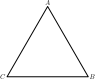
\includegraphics{triangle.pdf}
  \end{center}
  \begin{enumerate}
    \item Find an equation for the distributed force $w(x)$.
      % Answer
      \A{
        The diagram depicts a distributed force that increases linearly from
        the left end ($x=0$) to $x=2\,\mathrm{m}$ and is then zero until the
        end of the beam. We have then
        \[
          w(x) =
          \begin{cases}
            \frac{5}{2}\knewtons/\mathrm{m} \times x
              & \text{for } 0 \leq x \leq 2\metres \\
            0 & \text{for } 2\metres \le x \leq 5\metres
          \end{cases}
        \]
      }
    \item Find the total force and moment around $A$ of $w(x)$ and hence find
      the reactions $R_A$ and $M_A$.
      \A{
        \[
          F_w = \int_0^5 w(x)\dx{x}
              = \int_0^2 \frac{5}{2}x\dx{x} + \int_2^5 0\dx{x}
              = \left[\frac{5}{4}x^2\right]_0^2 = 5\knewtons
        \]
        \[
          M_w = \int_0^5 x w(x)\dx{x} = \frac{20}{3}\knewtons\mathrm{m}
        \]
        Hence $R_A = 5\knewtons$ and $M_A = -\frac{20}{3}\knewtons\mathrm{m}$.
      }
    \item If there were a point force equivalent to $w(x)$ (for external force
      and moment balance) what would it be and where would it act?
      \A{
        For force balance it would need to be a downwards force of
        $5\knewtons$. For moment balance it would need to be at $x =
        \frac{4}{3}\metres$.
      }
    \item Find the shear stress $V(x)$ and bending moment $M(x)$ throughout
      the beam. Verify that your solutions satisfy the correct boundary
      conditions at both ends of the beam.
      \A{
        For the shear stress we have $V'(x) = -w(x)$ with BCs $V(0)=R_A$ and
        $V(5)=0$. Starting from the left we have that
        \[
          V(x) = - \int w(x)\dx{x}
               = - \int \frac{5}{2}x\dx{x}
               = - \frac{5}{4}x^2 + C_1
               = 5\knewtons - \frac{5}{4}x^2
        \]
        for $0 \leq x \leq 2$ and where we have used the BC for $V(0)$. We can
        use this to find that $V(2) = 0$ which gives our BC for the next part.
        For $x > 2$ we have that $w(x)=0$ so $V(x) = C_2 = 0$ (since
        $V(2)=0$). Putting all this together we get
        \[
          V(x) =
          \begin{cases}
            5\knewtons - \frac{5}{4}\knewtons/\mathrm{m}^2 \times x^2
                & \text{for } 0 \leq x \leq 2\metres \\
            0   & \text{for } 2 < x \leq 5\metres
          \end{cases}
        \]
        and it is easy to see that this satisfies $V(5) = 0$.\newline
        For the bending moment we need to solve $M'(x) = V(x)$ with $M(0)=M_A$
        and $M(5) = 0$. This gives
        \[
          M(x) = \int w(x)\dx{x}
               = \int 5 - \frac{5}{4}x^2 \dx{x}
               = 5x - \frac{5}{12}x^3 + C_3
               = 5x - \frac{5}{12}x^3 - \frac{20}{3}\knewtons\mathrm{m}
        \]
        for $0 \leq x \leq 2\metres$ and where we have used the BC for $M(0)$.
        This gives $M(2) = 0$ as our BC for the next part. Since for $x > 2$
        the shear stress $V(x)=0$ we have that $M(x) = C_4 = 0$ (using our BC
        for $M(2)$). Finally we have
        \[
          M(x) =
          \begin{cases}
            5\knewtons \times x - \frac{5}{12}\knewtons/\mathrm{m}^2 \times x^3
                                - \frac{20}{3}\knewtons\mathrm{m}
                & \text{for } 0 \leq x \leq 2\metres \\
            0   & \text{for } 2 < x \leq 5\metres
          \end{cases}
        \]
        and it is easy to see that our BC for $M(5)$ is satisfied.
      }
  \end{enumerate}
}

\multiproblem{rectangle}{
  Repeat the above calculations for the rectangular load distribution shown
  here:
  \begin{center}
    \includegraphics{rectangle.pdf}
  \end{center}
  \A{
    Firstly we have
    \[
      w(x) =
        \begin{cases}
          0    & \text{for } 0 \leq x \leq \frac{L}{2} \\
          w_0  & \text{for } \frac{L}{2} < x \leq L
        \end{cases}
    \]
    We can integrate to find $R_A = \frac{1}{2}w_0 L$ and $M_A = -\frac{3}{8}
    w_0 L^2$.
  }

  \A{
    Then the shear stress for $x \leq \frac{L}{2}$ is given from
    $V'(x) = 0$ so that $V(x)=C_1=\frac{1}{2}w_0 L$ using the BC for $V(0)$.
    This gives that $V(\frac{L}{2}) = \frac{1}{2}w_0 L$ which is our BC for
    the second half. For $x > \frac{L}{2}$ we have $V'(x) = -w_0$ so $V(x) =
    -w_0 x + C_2 = w_0 (L - x)$ using the BC for $V(\frac{L}{2})$. Altogether
    then
    \[
      V(x) =
        \begin{cases}
          \frac{1}{2}w_0 L    & \text{for } 0 \leq x \leq \frac{L}{2} \\
          w_0 (L - x)         & \text{for } \frac{L}{2} < x \leq L
        \end{cases}
    \]
  }

  \A{
    We can similarly find that
    \[
      M(x) =
        \begin{cases}
          \frac{1}{2}w_0 L x - \frac{3}{8}w_0 L^2
              & \text{for } 0 \leq x \leq \frac{L}{2} \\
          -\frac{1}{2} w_0 (L - x)^2
              & \text{for } \frac{L}{2} < x \leq L
        \end{cases}
    \]
    and we can easily see that $V(L) = 0$ and $M(L) = 0$ as expected.
  }
}

\multiproblem{point}{
  Find the bending moment and shear stress throught the beam shown here:
  \begin{center}
    \includegraphics{point_distributed.pdf}
  \end{center}
  \A{
    Firstly we have that
    \[
      w(x) =
        \begin{cases}
          w_0 (\frac{x}{2d} - 1)  & \text{for } 2d \leq x \leq 4d \\
          0 & \text{otherwise}.
        \end{cases}
    \]
    Force balance and moment balance around $A$ gives $R_A = F_0 + w_0 d$ and
    $M_A = -F_0 d - \frac{10}{3}w_0 d^2$.
  }

  \A{
    To find the shear stress we will work from left to right handling the
    three sections separately. For $0 \leq x < d$ we have $w(x) = 0$ so
    \[
      V(x) = C_1 = R_A = F_0 + w_0 d.
    \]
    We know that the shear stress must satisfy $V_-(d) = V_+(d) + F_0$ so
    $V_+(d) = w_0 d$ which gives the BC for the next part. Then for $d < x
    \leq 2d$ we have $w(x)=0$ again so
    \[
      V(x) = C_2 = V_+(d) = w_0 d
    \]
    which also now gives us that $V(2d) = w_0 d$. Finally for $2d < x \leq 4d$
    we have $w(x) = w_0 (\frac{x}{2d} - 1)$ so
    \[
      V(x) = - \int w_0  \left(\frac{x}{2d}   - 1\right) \dx{x}
           = - w_0 \left(\frac{x^2}{4d} - x\right) + C_3
           = - w_0 \left(\frac{x^2}{4d} - x\right)
           = w_0 \left(x - \frac{x^2}{4d}\right)
    \]
    where we have used the BC for $V(2d)$ to find $C_3$. Putting this
    altogether we find that the shear stress is given by
    \[
      V(x) =
        \begin{cases}
          F_0 + w_0 d               & \text{for } 0 \leq x < d \\
          w_0 d                     & \text{for } d < x \leq 2d \\
          w_0 \left(x - \frac{x^2}{4d}\right) & \text{for } 2d < x \leq 4d
        \end{cases}.
    \]
    and it is easy to check that the BC $V(4d) = 0$ is satisfied.
  }

  \A{
    To find the bending moment we need to integrate $V(x)$ which we now have a
    rather complicated expression for. For $0 \leq x \leq d$ we have
    \[
      M(x) = (F_0 + w_0 d)x + C_4
           = (F_0 + w_0 d) x - F_0 d - \frac{10}{3}w_0 d^2
           = F_0 (x - d) + w_0 d \left(x - \frac{10}{3}d\right)
    \]
    which gives that $M(d) = -\frac{7}{3} w_0 d^2$. For $d \leq x \leq 2d$ we
    get that
    \[
      M(x) = w_0 d x + C_5
           = w_0 d \left(x - \frac{10}{3}d\right)
    \]
    which gives that $M(2d) = -\frac{4}{3}wd^2$. Finally for $2d \leq x \leq
    4d$ we have that
    \[
      M(x) = \int w_0 \left(x - \frac{x^2}{4d}\right) \dx{x}
           = w_0 \left(\frac{x^2}{2} - \frac{x^3}{12d} \right) + C
           = w_0 \left(\frac{x^2}{2} - \frac{x^3}{12d} - \frac{8}{3}d^2\right).
    \]
    Putting this all together we find that
    \[
      M(x) =
        \begin{cases}
          F_0 (x - d) + w_0 d \left(x - \frac{10}{3}d\right)
                & \text{for } 0 \leq x < d \\
          w_0 d \left(x - \frac{10}{3}d\right)
                & \text{for } d < x \leq 2d \\
          w_0 \left(\frac{x^2}{2} - \frac{x^3}{12d} - \frac{8}{3}d^2\right)
                & \text{for } 2d < x \leq 4d.
        \end{cases}.
    \]
    and we can easily check that this satisfies $M(4d) = 0$.
  }
}

\multiproblem{diving}{
  Consider this arrangement:
  \begin{center}
    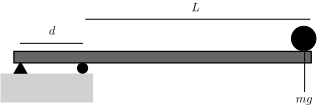
\includegraphics{diving.pdf}
  \end{center}
  \begin{enumerate}
    \item Find the reaction forces at the two supports resulting from the
      large weight at the end of the beam (assume the beam has zero mass).
      \A{
        Force balance gives that $R_A+R_B = mg$. Taking moments around the
        middle support ($B$) gives that $mgL + R_A d = 0$ so we have $R_A =
        -\frac{mgL}{d}$ and $R_B = mg\left(1 + \frac{L}{d}\right)$.
      }
    \item Find shear stress and bending moment throughout the length of the
      beam.
      \A{
        Divide into $x < d$ and $d < x < d + L$. For $x < d$ we have $V'(x)=0$
        so $V(x) = C_1 = R_A = -\frac{mgL}{d}$ so $V_-(0) = -\frac{mgL}{d}$. The
        point force at $B$ gives us that $V_-(0) = V_+(0) + R_B$ so $V_+(0) =
        mg$. We also have $V'(x)=0$ for $x > d$ so this gives
        \[
          V(x) =
          \begin{cases}
            -\frac{mgL}{d} & \text{for } 0 < x < d \\
            mg             & \text{for } d < x < d + L \\
          \end{cases}
        \]
        which satisfies the BC at the right hand side ($V(d+L) = mg$).
      }

      \A{
        The bending moment is given by $M'(x) = V(x)$ with $M(0) = M(d+L)=0$
        so we have
        \[
          M(x) =
          \begin{cases}
            -\frac{mgL}{d}x & \text{for } 0 < x < d \\
            mg(x-d-L)             & \text{for } d < x < d + L \\
          \end{cases}
        \]
      }
    \item Repeat the calculations taking account of the weight of the beam.
      Assume it has mass $m_b \neq 0$.
      \A{
        Force balance now gives $R_a+R_B = (m + m_b) g$. Moment balance around
        $A$ gives
        \[
          dR_A + mg L + m_B g \frac{L - d}{2}
        \]
      }
  \end{enumerate}
}

\multiproblem{bridge}{
  Repeat the above calculations for this bridge (both for zero and non-zero
  beam mass):
  \begin{center}
    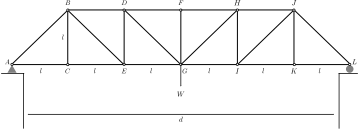
\includegraphics{bridge.pdf}
  \end{center}
}
